\documentclass{beamer}
%[aspectratio=169]   \usepackage[czech]{babel}
\usepackage{apo-lecture-en}
\usepackage{pdfpages}
\usepackage{pdfcomment}
\usepackage{listings}
\usepackage{array,multirow}

\subtitle{Lecture 02. Integer and Floating Point Numbers}
\author{Pavel Píša \phantom{xxxxxxxxx} Petr Štěpán \\ \small\texttt{pisa@fel.cvut.cz} \phantom{xx} \small\texttt{stepan@fel.cvut.cz} \\
\phantom{xxxxxxxxx} \\
License: CC-BY-SA}
\begin{document}

\maketitle

\section{Integer Numbers and Operations}

\begin{frame}
\frametitle{Repetition and Fundamentals from Previous Lecture}
The last lecture introduced:
\begin{itemize}
\item The bit (logical value) representation by voltage level
\item Byte (logical values vector) representation using parallel bit signals/wires/conductors
\item To represent arithmetic unsigned integer values, weights of power two are assigned to the parallel signals
\item Positional (place-value) notation / numeral system is introduced
\item The representation has been used to implement operation of addition of two non-negative numbers
\item Logical bit shift has been introduced (it is correspondent to multiply and divide by power of two for binary number representation)
\end{itemize}
\end{frame}


\begin{frame}
\frametitle{The Current Lecture Topics}
\begin{itemize}
\item The ranges which can be represented by integer numbers and their storage in memory
\item Multiplication and division of integer non-negative numbers
\item Signed numbers (range split for negative part) and respective operation
\item Arithmetic and unsigned overflow
\item Real numbers representation and operations
\end{itemize}
\end{frame}


\begin{frame}
\frametitle{Quiz 1}
How fast can the sum of two n-bit numbers be calculated, and how many transistors do we need?
\begin{itemize}
\item[A] in constant time ($O(1)$) with linear number of transistors ($O(n)$)
\item[B] in constant time ($O(1)$) with exponential number of transistors ($O(2^n)$)
\item[C] in logarithmic time ($O(\log{n})$) with linear number of transistors ($O(n)$)
\item[D] in logarithmic time ($O(\log{n})$) with cubic number of transistors ($O(n^3)$)
\item[E] in logarithmic time ($O(\log{n})$) with exponential number of transistors ($O(2^n)$)
\end{itemize}
\end{frame}


\begin{frame}
\frametitle{Non-negative Integer Numbers}
Non-negative integer numbers representation

C-language standard (ISO/IEC 9899:TC3) defines:
\begin{tabular}{|l|r|r|c|}\hline
type & min & max & informative bytes\\ \hline
unsigned char & 0 & 255 & 1 \\ \hline
unsigned short & 0 & 65 535 & 2 \\ \hline 
unsigned long & 0 & 4 294 967 295 & 4 \\ \hline
unsigned long long & 0 & 18 446 744 073 709 551 615 & 8 \\ \hline
\end{tabular}

\begin{itemize}
\item The standard defines minimal ranges, \texttt{unsigned int} at least $2^{16}-1$ (2 bytes), but usually 4 bytes today.
\item To find actual size in basic addressable units (C char) use \texttt{sizeof(int)}, for range \texttt{UINT\_MAX}
\item For exact size use \texttt{uintX\_t} and \texttt{intX\_t} (where \texttt{X} is 8, 16, 32, or 64), i.e. \texttt{uint8\_t}, \texttt{int64\_t}
\item Some exact size types can be missing but guaranteed \texttt{[u]int\_fastX\_t} and \texttt{[u]int\_leastX\_t}, i.e. \texttt{uint\_least8\_t}, \texttt{int\_fast64\_t}
\end{itemize}

\end{frame}


\begin{frame}
\frametitle{Non-negative Integer Numbers in C-Language}
The constant values (integer literal) in C-language source:
\begin{itemize}
\item decimal number -- has to start by digit '1' to '9' except for '0'
\item octal number -- starts by digit '0'
\item hexadecimal -- starts by '0x', continues by '0' -- '9' and 'a' to 'f'
\item binary -- starts by '0b' (GNU compiler extension / C++14 / C23)
\end{itemize}
\bigskip
Example: 252 == 0xfc == 0374 == 0b11111100
\bigskip

Remark: The hexadecimal digits mapping to bytes is straightforward, each digit (nibble) represents four bits and two digits expressed number fits into single byte, i.e. 0x123456 fits into three bytes (24 bits rounded, exact minimum 21 bits)
\end{frame}


\begin{frame}
\frametitle{Non-negative Integer Numbers in Memory}

\begin{itemize}
\item Computer memory works with addressable units/cells (usually bytes)
\item There are the two basic options for storing longer numbers in memory.
\end{itemize}

The number 0x12345678 for fixed sized integer types (unsigned int):
\begin{tabular}{|c|c|c|}\hline
address & Big-endian & Little-endian \\ \hline
400 & 0x12 & 0x78 \\ \hline
401 & 0x34 & 0x56 \\ \hline
402 & 0x56 & 0x34 \\ \hline
403 & 0x78 & 0x12 \\ \hline
\end{tabular}

\begin{itemize}
\item Motorola and IBM processors started with big-endian, Intel processors are usually little-endian.
\item It's important when you read/receive (Internet) serialized data by bytes, for example, you have to agree on order between systems
\item RISC V - little-endian, MIPS - big-endian but later even little-endian
\item Bitcoin - DER signatures big-endian, transaction hash-endian
\end{itemize}
\end{frame}


\begin{frame}[fragile]
\frametitle{Non-negative Integer Numbers -- Quiz 2}
\begin{minted}{c}
#include <stdio.h>
int main() {
  unsigned char p[] = {0,0,0,0};
  *(int*)p=10;
  printf("%02x,%02x,%02x,%02x\n", p[0],p[1],p[2],p[3]);
}
\end{minted}

What is the output of the above program on Intel processors?
\begin{itemize}
\item[A] nothing, the code cannot be translated
\item[B] random result, p (unsigned char *) cannot be casted to *int
\item[C] 0a,00,00,00 
\item[D] 00,00,00,0a
\end{itemize}
\end{frame}



\begin{frame}
\frametitle{Non-negative Integer Number Multiplication}

The same principle which you have learned at basic school for decimal numeral system
\begin{columns}
\begin{column}{0.4\textwidth}
\texttt{\phantom{xxx}153\phantom{xx}}\\
\texttt{\phantom{xxx}*45\phantom{xx}}\\
\vspace{-8pt}
\rule[0pt]{1.5cm}{0.1pt}\\
\texttt{\phantom{xxx}765\phantom{x}5}\\
\texttt{\phantom{xx}612\phantom{xx}4}\\
\vspace{-8pt}
\rule[0pt]{1.5cm}{0.1pt}\\
\texttt{\phantom{xx}6885\phantom{xx}}\\
\end{column}
\hfill
\begin{column}{0.4\textwidth}
\texttt{\phantom{xxxxxx}10011001\phantom{xx}}\\
\texttt{\phantom{xxxxxxx}*101101\phantom{xx}}\\
\vspace{-8pt}
\rule[0pt]{3cm}{0.4pt}\\
\texttt{\phantom{xxxxxx}10011001\phantom{x}1}\\
\texttt{\phantom{xxxxx}00000000\phantom{xx}0}\\
\texttt{\phantom{xxxx}10011001\phantom{xxx}1}\\
\texttt{\phantom{xxx}10011001\phantom{xxxx}1}\\
\texttt{\phantom{xx}00000000\phantom{xxxxx}0}\\
\texttt{\phantom{x}10011001\phantom{xxxxxx}1}\\
\vspace{-8pt}
\rule[0pt]{3cm}{0.4pt}\\
\texttt{\phantom{x}1101011100101\phantom{xx}}\\
\end{column}
\end{columns}

\end{frame}


\begin{frame}
\frametitle{Sequential Integer Number Multiplication}

The realization of the algorithm form previous slide with shift register and adder:\\
(inputs A,B 32-bit, result 64-bit)
\begin{center}

\includegraphics[width=0.55\textwidth]{multiplier-seq-en.pdf}
\end{center}
\begin{itemize}
\item The result will be available after 32 cycles in AC and B 
\item It is slow, even adder and addition required 32 times (64 times for 64-bit systems).
\end{itemize}
\end{frame}


\begin{frame}
\frametitle{Fast Multiplication -- Wallace Tree Motivation}

Potential for speedup -- delayed carry (Carry Save Adder).\\
The optimization of the sum of four 32-bit integers:\\
\begin{columns}
\begin{column}{0.35\textwidth}
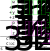
\includegraphics[width=1.0\textwidth]{wallace-tree.pdf}
\end{column}
\hfill
\begin{column}{0.65\textwidth}
\begin{itemize}
\item r=w+x and s=y+z can be computed in parallel and then is computed r+s -- time equivalent to two full additions
\item The carry chain can be delayed (carry is not propagated until the last step):
\begin{itemize}
\item step 1 -- use unchained \texttt{full adder}s and proceed $w_i+x_i+y_i = c'_ip_i$
\item step 2 -- use \texttt{full adder}s again for bits $p_i+c'_{i-1}+z_i = c_iq_i$
\item step 3 -- regular adder (i.e. CLA) for 32-bit numbers ($s_0=q_0$, $c'_32$ added to $q$)
\end{itemize}
\end{itemize}
\end{column}
\end{columns}
\end{frame}


\begin{frame}
\frametitle{Fast Multiplication -- Wallace Tree}

Try to apply the described principle to sum fast 32 or 64 values:
\begin{columns}
\begin{column}{0.6\textwidth}

\includegraphics[width=1.0\textwidth]{wallace-tree2.pdf}
\end{column}
\hfill
\begin{column}{0.4\textwidth}
\begin{itemize}
\item Actual one bit multiplication is trivial: $x_i \cdot y_j=x_i$~\texttt{and}~$y_j$
\item The most demanding is to sum central column with 64 single bit values
\item The adders will be run in parallel on all bits which map to their three inputs and carry will be processed in following steps
\item The first phase requires 1323 adders
\end{itemize}
\end{column}
\end{columns}

\end{frame}


\begin{frame}[shrink=5]
\frametitle{Fast Multiplication -- Wallace Tree}

The longest, central column in more detail:
\begin{center}
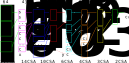
\includegraphics[width=0.8\textwidth]{wallace-tree3.pdf}
\end{center}

\begin{itemize}
\item After 8 counting steps, i.e. 16 gate delays, the two bits are ready for final adder
\item The column on the right of the central one are already partially summed and 8 the last carry signals have been promoted
\item Two 120-bit numbers (sum and carry) remain to add, which can also be done in 30 gate delays
\item Result - we multiply two numbers for the price of time corresponding to two 64-bit additions
\end{itemize}

\end{frame}


\begin{frame}
\frametitle{Sequential Integer Number Division}

Division in the binary system can be done the same way as manual decimal division:
\bigskip
\begin{columns}
\begin{column}{0.4\textwidth}
\texttt{\phantom{-}240:11=21}\\
\texttt{-22}\\
\vspace{-8pt}
\rule[0pt]{1cm}{0.1pt}\\
\texttt{\phantom{xx}20}\\
\texttt{\phantom{x}-11}\\
\vspace{-8pt}
\rule[0pt]{1cm}{0.1pt}\\
\texttt{\phantom{xxx}9}\\
\end{column}
\hfill
\begin{column}{0.4\textwidth}
\texttt{\phantom{x}11110000:1011=10101}\\
\texttt{-1011}\\
\vspace{-8pt}
\rule[0pt]{1cm}{0.4pt}\\
\texttt{\phantom{xx}1000}\\
\texttt{\phantom{xx}10000}\\
\texttt{\phantom{xx}-1011}\\
\vspace{-8pt}
\rule[0pt]{1.4cm}{0.4pt}\\
\texttt{\phantom{xxxx}1010}\\
\texttt{\phantom{xxxx}10100}\\
\texttt{\phantom{xxxx}-1011}\\
\vspace{-8pt}
\rule[0pt]{1.8cm}{0.4pt}\\
\texttt{\phantom{xxxxx}1001}\\
\end{column}
\end{columns}
\bigskip
The both evaluation of 240 by 11 result in 21 and the remainder is \texttt{240\%11=9}.

\end{frame}


\begin{frame}
\frametitle{Sequential Integer Number Division}

The \texttt{A/B} operation, A is 64-bit, B is 32-bit:

\begin{columns}
\begin{column}{0.45\textwidth}
The input A is stored into two registers AC,A\\

\includegraphics[width=1\textwidth]{divider-seq-en.pdf}
\end{column}
\hfill
\begin{column}{0.55\textwidth}
\begin{itemize}
\item Result: A register integral ratio, AC reminder -- modulo
\item The A register is shifted only in the last step, AC is not shifted -- why?
\item There exists an even faster algorithm -- High Radix Division (it is complex, above focus of our subject)
\begin{itemize}
\item It estimates more bits by approximation and iteration to enhance precision follows
\item 1994 -- Pentium FDIV bug -- incorrect implementation of Sweeney, Robertson, and Tocher (SRT) algorithm -- two bits estimated per single cycle
\end{itemize}
\end{itemize}
\end{column}
\end{columns}


\end{frame}


\section{Signed Numbers}

\begin{frame}
\frametitle{Signed Numbers -- Way to Include Negative Ones}

The sign has to be encoded into numeral representation:
\begin{itemize}
\item simple way - the most significant bit represents sign
\begin{itemize}
\item The absolute value the rest but 0 and -0 even that represents the same value
\item The addition complicated and unsigned adder is hard to reuse
\end{itemize}
\item two's complement (complement to module) -- most frequent in use
\begin{itemize}
\item the $X$ arithmetic value representation by k-bit binary evaluates to $X$ \texttt{mod} $2^k$
\begin{itemize}
\item if $X\ge0$, the representation is the same $X$
\item if $X<0$, the value is represented by $2^k-|X|$
\end{itemize}
\item advantages: the exactly same adder can be used for signed and unsigned types.
\end{itemize}
\begin{itemize}
\item -1 represented by 8-bit two's complement binary \texttt{11111111}
\item 5+(-1) is \texttt{101+11111111=\textcolor{red}{1}00000100}, the bit 8 (9-th) does not fit into representation, so the results is \texttt{101+11111111=100}, i.e. 4 in decimal
\end{itemize}
\end{itemize}


\end{frame}

\begin{frame}
\frametitle{Two's Complement (Complement to Module)}
\begin{itemize}
\item the k bits can represent the range $<-2^{k-1}, 2^{k-1}-1>$
\item let X is arithmetic value, A(X) is unsigned binary value in the two's complement:
\end{itemize}
\vspace{-0.3cm}
\begin{columns}
\begin{column}{0.5\textwidth}

\includegraphics[width=0.9\textwidth]{doplnek-graf.pdf}
\end{column}
\hfill
\begin{column}{0.5\textwidth}
\begin{tabular}{|c|c|}\hline
{\small 8-bit A(X)}  & {\small Arithmetic value} \\\hline
\textbf{0}0000000 & $0_{(10)}$ \\ \hline
\textbf{0}0000001 & $1_{(10)}$ \\ \hline
... & ... \\\hline
\textbf{0}1111110 & $126_{(10)}$ \\ \hline
\textbf{0}1111111 & $127_{(10)}$ \\ \hline
\textbf{1}0000000 & $-128_{(10)}$ \\ \hline
\textbf{1}0000001 & $-127_{(10)}$ \\ \hline
\textbf{1}0000010 & $-126_{(10)}$ \\ \hline
... & ... \\\hline
\textbf{1}1111101 & $-3_{(10)}$ \\ \hline
\textbf{1}1111110 & $-2_{(10)}$ \\ \hline
\textbf{1}1111111 & $-1_{(10)}$ \\ \hline
\end{tabular}
\end{column}
\end{columns}
\end{frame}


\begin{frame}
\frametitle{Additive Inverse (Opposite Number)}
\begin{itemize}
\item The addition of the numbers represented by the two's complement is same as for non-negative ones and subtraction \texttt{A-B} can be realized as addition where inverse of \texttt{B} is added, i.e. \texttt{A+(-B)}
\item The idea how to compute inverse (often \texttt{neg} instruction) \texttt{-B} from \texttt{B} comes from
\begin{itemize}
\item two's complement negative values are encoded as $X = 2^k-|X|$
\item if we negate (complement) each bit individually we get $(2^{k}-1)-X$, because $2^{k}-1$ is represented by $k$ ones, no borrow from more significant bits are required
\end{itemize}
\item Final algorithm is:
\begin{enumerate}
\item negate, complement all bits of the input $X$
\item add one to the result
\end{enumerate}
\end{itemize}

Example:\\
\texttt{53=0b00110101} bit complement gives \texttt{-54=0b11001010} and result after addition of one is \texttt{-53=0b11001011}

\end{frame}


\begin{frame}
\frametitle{Integer Subtraction}


\begin{columns}
\begin{column}{0.5\textwidth}
It can be solved:
\begin{itemize}
\item by a special circuit similar to an addition with all acceleration possibilities as for addition
\item or from the two's complement and inverse number we can convert it to addition and same hardware
\end{itemize}
\end{column}
\hfill
\begin{column}{0.5\textwidth}
\begin{center}

\includegraphics[width=0.5\textwidth]{substaction-en.pdf}
\end{center}
\end{column}
\end{columns}


\end{frame}

\begin{frame}
\frametitle{Single Unit for Addition and Subtraction}


\begin{center}

\includegraphics[width=0.5\textwidth]{add-sub-en.pdf}
\end{center}

\end{frame}


\begin{frame}
\frametitle{Multiplication and Division in Two's Complement}

\begin{itemize}
\item rule for adjustment of the result of multiplication based on unsigned $M\cdot N$, ($A(M)\cdot A(N)$) multiplication of two $M$, $N$ two's complement k-bit numbers :

\end{itemize}
$A(M\cdot N) = A(M) \cdot A(N)$\\
\phantom{$A(M\cdot N)$ }$-A(M) \cdot 2^k$ \phantom{xxxxx} when $M<0$\\
\phantom{$A(M\cdot N)$ }$-A(N) \cdot 2^k$ \phantom{xxxxx} when $N<0$
%\begin{itemize}
\begin{itemize}
\item because two's complement representation of $A(M) = 2^k+M$, then result of multiplication for for two negative numbers is $(2^k+M)\cdot (2^k+N) = 2^{2\cdot k}+2^k \cdot M + 2^k \cdot N + M \cdot N$
\end{itemize}
%\end{itemize}
\begin{itemize}
\item today's fast multipliers and divisors compute usually with absolute values and for the sign
\begin{itemize}
\item it is stored in the most significant bit
\item inverse number computation is fast
\end{itemize}
\end{itemize}
\end{frame}


\begin{frame}
\frametitle{Signed Numbers in C-language}
Integer numbers representation in C

Next types are defined by standard with minimal ranges:
\begin{tabular}{|l|r|r|c|}\hline
type & min & max & byte count\\ \hline
char & -128 & 127 & 1 \\ \hline
short & -32 768 & 32 767 & 2 \\ \hline 
long & -2 147 483 648 & 2 147 483 647 & 4 \\ \hline
long long & -9 223 372 036 & 9 223 372 036  & 8 \\ 
 & \phantom{xx} 854 775 808 & \phantom{xx}854 775 807 &  \\ \hline
\end{tabular}

\begin{itemize}
\item The C standard defines required minimum by one higher than two's complement to not eliminate processor computing in one's complement -- but that is not practically used today
\item To be sure about actual range of \texttt{int} use \texttt{INT\_MIN} and \texttt{INT\_MAX}
\end{itemize}

\end{frame}


\begin{frame}[fragile, shrink=5]
\frametitle{Signed Numbers -- Quiz 3}

Consider the following program:
\begin{minted}{c}
#include <stdio.h>
int main() {
  unsigned char a=150u, b=120u, c;
  char sa=-100, sb=-80, sc;
  
  c=a+b;
  sc=sa+sb;
  printf("c=%u sc=%d\n", c, sc);
}
\end{minted}

What will be printed:
\begin{itemize}
\item[A] c=270 sc=-180
\item[B] c=14 sc=-76
\item[C] c=14 sc=76
\item[D] c=-14 sc=-76
\item[E] Numeric error
\end{itemize}
\end{frame}

\begin{frame}
\frametitle{Overflow for Unsigned Numbers}


Unsigned char is 8-bit represented number typically which is reason that next operation overflows:\\
\texttt{\phantom{x}150 = \phantom{x}1001 0110}\\
\texttt{+120 = \phantom{x}0111 1000}\vspace{-6pt}\\
\rule[0pt]{3.6cm}{0.4pt}\\
\texttt{\phantom{xx}14 = \phantom{x}0000 1110}\\
\texttt{\phantom{x}270 =1 0000 1110}

The result does not fit in 8-bit representation, the most significant bit is lost, and the result is only 14.

If we want to signal overflow in addition we can use:
\begin{itemize}
\item C23 bool ckd\_add(type1 *result, type2 a, type3 b) -- addition of two numbers with overflow signalling
\item GNU GCC 5+, Clang 3.8+ \_\_builtin\_add\_overflow(a, b, result) -- both versions even for sub and mul
\item Can be detected on conventional C by check if the result is smaller than both inputs
\end{itemize}
\end{frame}

\begin{frame}
\frametitle{Arithmetic Overflow for Signed Numbers}

The overflow in operations with signed numbers is more complex. Examples what results in overflow:
\bigskip
\begin{columns}
\begin{column}{0.3\textwidth}
\texttt{-112 = 10010000}\\
\texttt{+\phantom{x}45 = 00101101}\\
\vspace{-8pt}
\rule[0pt]{3cm}{0.1pt}\\
\texttt{\phantom{x}-67 = 10111101}\\
\begin{center}
\large CORRECT
\end{center}
\end{column}
\hfill
\begin{column}{0.3\textwidth}
\texttt{\phantom{xx}-12 = 11110100}\\
\texttt{+ -20 = 11101100}\\
\vspace{-8pt}
\rule[0pt]{3cm}{0.1pt}\\
\texttt{\phantom{xx}-32 =\textcolor{red}{1}11100000}\\
\begin{center}
\large CORRECT
\end{center}
\end{column}
\hfill
\begin{column}{0.3\textwidth}
\texttt{\phantom{xx}-90 = 10100110}\\
\texttt{+ -42 = 11010110}\\
\vspace{-8pt}
\rule[0pt]{3cm}{0.1pt}\\
\texttt{\phantom{xx}124 =\textcolor{red}{1}01111100}\\
\begin{center}
\large OVERFLOW
\end{center}
\end{column}
\end{columns}
\bigskip
\begin{itemize}
\item The arithmetic overflow for operation with signed numbers is present if auxiliary carry to the most significant result bit differs from the carry out from this bit:
\begin{itemize}
\item overflow = $c_n$ xor $c_{n-1}$; $c_n$ carry from most significant result bit, $c_{n-1}$ is carry into the most significant bit
\end{itemize}
\item The second option i to check that addition result of the two positive numbers is positive and for two negative numbers stay negative:
\begin{itemize}
\item overflow = ($a_{n-1}$ and  $b_{n-1}$ and (not $s_{n-1}$)) or ((not $a_{n-1}$) and  (not $b_{n-1}$) and $s_{n-1}$); $a_{n-1}$, $b_{n-1}$ are the most significant bits of addends; $s_{n-1}$ is MSB of result
\end{itemize}
\end{itemize}
\end{frame}

\begin{frame}
\frametitle{Arithmetic Overflow -- Quiz 4}

\begin{center}

\includegraphics[width=0.6\textwidth]{overflow.pdf}
\end{center}

When two numbers with opposite signs are added:
\begin{itemize}
\item[A] can only overflow in two's complement representation
\item[B] can only overflow in representation other two's complement representation
\item[C] cannot only occur in representation in two's complement representation
\item[D] cannot occur in any representation of signed numbers
\end{itemize}
\end{frame}



\begin{frame}
\frametitle{Other Representations of Signed Numbers}

Excess-K (offset binary):

\begin{columns}
\begin{column}{0.5\textwidth}
\begin{itemize}
\item for k-bit representation, offset K is usually $K=2^{k-1}$ or $K=2^{k-1}-1$
\item representation/code for number X is $A(X) = X+K$
\item arithmetic value is obtained from $D(A) = A-K$
\item the range of the represented arithmetic values is $<-K, 2^{k}-K-1>$
\end{itemize}
\end{column}
\hfill
\begin{column}{0.5\textwidth}
for k=8 and K=127
\bigskip
\begin{tabular}{|c|c|}\hline
{\small A(X)}  & {\small Value} \\\hline
00000000 & $-127_{(10)}$ \\ \hline
00000001 & $-126_{(10)}$ \\ \hline
... & ... \\\hline
01111110 & $-1_{(10)}$ \\ \hline
01111111 & $0_{(10)}$ \\ \hline
10000000 & $1_{(10)}$ \\ \hline
10000001 & $2_{(10)}$ \\ \hline
... & ... \\\hline
11111110 & $127_{(10)}$ \\ \hline
11111111 & $128_{(10)}$ \\ \hline
\end{tabular}
\end{column}
\end{columns}

\end{frame}

\begin{frame}
\frametitle{Excess-K -- Arithmetic Operations}

\begin{itemize}
\item the addition and subtraction operations processed directly representation:
\item $A ( X + Y )=( X + Y )+ K =( X + K ) + (Y + K ) - K = A ( X )+ A (Y ) -K$
\item $A ( X - Y )=( X - Y )+ K =( X + K ) - (Y +K )+K = A ( X ) - A (Y )+K$
\item multiplication is even more complex:
\item $A ( X \cdot Y )=( X \cdot Y )+K =( X + K )\cdot(Y + K )-( X + K +Y +K )\cdot K + K^2+ K
= A ( X )\cdot A (Y ) - ( A ( x)+ A ( y ))\cdot K + K^2 +K$
\end{itemize}
\bigskip
\begin{itemize}
\item Overflow:
\begin{itemize}
\item for addition, same sign inputs and opposite sign on output
\end{itemize}
\end{itemize}
\end{frame}


\begin{frame}
\frametitle{Other Representations of Signed Numbers}

One's complement:
\begin{itemize}
\item negative number is represented by bit complement of its absolute value. For k-bit representation:
\begin{itemize}
\item for $X\ge0$, representation is $A(X) = X$
\item for $X<0$, representation is $A(X) = 2^k-1-|X|$
\end{itemize}
\item disadvantages: two representations of the value zero (-0, +0) complicate addition (hot one correction)
\end{itemize}
\bigskip
Binary coded decimal (BCD) representation
\begin{itemize}
\item another representation of integer numbers, each decimal digit maps to nibble 
\begin{itemize}
\item the number \texttt{1234} representation printed in hexadecimal form gives \texttt{0x1234}
\end{itemize}
\item advantages: simple conversion to and from decimal input/output
\item disadvantages: ineffective storage -- space waste, complex computation
\end{itemize}
\end{frame}


\section{Real Numbers}


\begin{frame}
\frametitle{Real Numbers}

\begin{itemize}
\item Integer number $X$ in $k$-bit binary representation can be split into bits where each $b_i$ is multiplied by corresponding power of two (weight), that is $ X = \sum_{i=0}^{k-1} b_i 2^{i} $
\item Real number $X$ is again similar sum of $k+j$ bits $b_i$ which are multiplied by powers of two (2), but we add negative powers of two: $X = \sum_{i=-j}^{k} b_i 2^{i}$
\item Remember grammar school math lessons $2^{-j} = \frac{1}{2^j}$
\end{itemize}


\begin{center}

\includegraphics[width=0.65\textwidth]{float_bin-1.pdf}
\end{center}

\end{frame}


\begin{frame}
\frametitle{Fixed Point Real Numbers}

Fixed point numbers:

\begin{itemize}
\item similar as signed excess-K representation
\item real number is represented by k-bit signed integer number, the fixed number of fractional bits is chosen, where $0 \le s \le k$
\item representation for arithmetic value X is $A(X) = \lceil X \cdot 2^s \rceil$
\item decoding of the representation to arithmetic value $D(A) = \frac{A}{2^s}$
\item the range of represented numbers $\langle -\frac{2^{k-1}}{2^s}, \frac{2^{k-1}-1}{2^s} \rangle$
\item absolute precision of the representation is $\pm \frac{1}{2^s}$.
\end{itemize}

 Special case for fractional numbers:
\begin{itemize}
\item if numbers from range $\langle 0,1)$ should be represented (usually control systems)
\item ten $s=k$ and we can directly use unsigned integer numbers representation
\item the better precision can be achieved than for the same bit size \texttt{float}, or \texttt{double} representation
\end{itemize}

\end{frame}

\begin{frame}
\frametitle{Fixed Point Real Numbers -- Operations}

\begin{itemize}
\item addition and subtraction is equivalent to the same operation on the number representation
\item multiplication requires fix-up (normalization) step:
\begin{itemize}
\item $A(X \cdot Y) = (X \cdot Y ) \cdot 2^s = \frac{(X \cdot 2^s)\cdot( Y\cdot 2^s) }{2^s} = \frac{A(X) \cdot A(Y)}{2^s}$
\end{itemize}
\item division is similar:
\begin{itemize}
\item $A(\frac{X}{Y}) = (\frac{X}{Y}) \cdot 2^s = \frac{(X \cdot 2^s)\cdot2^s }{( Y\cdot 2^s)} = \frac{A(X) \cdot 2^s}{A(Y)}$
\end{itemize}
\item It is not so significant complication because multiplication by $2^s$ is shift by $s$ bits to the left and division by $2^s$ is (arithmetic) shift by $s$ to the right.
\end{itemize}

\bigskip

Some SIMD instructions set extensions provide implementation of operations for computation in fixed point numbers representation.

\end{frame}


\begin{frame}
\frametitle{Floating Point Real Numbers }

\bigskip

It is equivalent to scientific notation format for decimal real numbers writing:
$-123 000 000 000 000.0 = -1.23 \cdot 10^{14} = -1.23\text{E} 14$\\
$-0.000 000 000 000 123 = -1.23 \cdot 10^{-13} = -1.23\text{E}-13$\\
Significand (mantissa) $\in \left\langle 1; 10 \right)$ for normalized form
\bigskip

Binary representation only changes base for exponent to 2:\\
$110 1100 0000 0000.0_2 = 1.1011_2 \cdot 2^{14} = 1.1011_2\text{E} 14 = 29696_{10}$\\
$-0.0000 0000 0000 0001 1101_2 = -1.1101_2 \cdot 2^{-16} = -1.1101_2\text{E}-16 \approx$\\
\phantom{xxxxxxxxxxxxxxxxxxxxxxxxxxxxxxxxxxxxxxxxxxxx}$\approx0.00002765_{10}$\\
Significand (mantissa) $\in \left\langle 1; 10_2 \right)$ that is
$\in \left\langle 1; 2_{10} \right)$ for normalized form
\bigskip

As in scientific notation the number has to start by single non-zero digit before decimal point, the binary representation has to start by single one (exception is zero) before binary point


\end{frame}

\begin{frame}
\frametitle{IEEE-754 Floating Point Standard}

Standard IEEE-754 defines how to encode real numbers into 32 (C float), 64 bits (C double)

32-bit representation of the real number composes of:
\begin{itemize}
\item 1 bit for the sign (both +0 and -0 are defined)
\item 8 bits two based exponent in excess-k representation (K=127)
\item 23 bits to represent significand fractions (plus implicit MSB one)
\end{itemize}
\bigskip
64-bit representation of the real number composes of:
\begin{itemize}
\item 1 bit sign (both +0 and -0 are defined)
\item 11 bits two based exponent in excess-k representation (K=1023)
\item 52 bits to represent significand fractions (plus implicit MSB one)
\end{itemize}

\end{frame}


\begin{frame}
\frametitle{IEEE-754}

Example:
Real number $0.828125_{(10)} = 0.5+0.25+0.0625+0.015625=2^{-1}+2^{-2}+2^{-4}+2^{-6} = 0.110101_{(2)}$.\\
The number is converted into scientific like binary format: $0.110101 = 1.10101\text{E}-1$.\\
Exponent is $e=-1$, its excess-k representation (K = 127) is $A(-1)=-1+127 = 126$.\\
The space for leading MSB of significand (hidden one)
is not reserved because it is guaranteed by format definition (except for zero and some corner cases):

\begin{center}
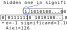
\includegraphics[width=0.4\textwidth]{float_example-en.pdf}
\end{center}

You can experiment with \url{https://www.h-schmidt.net/FloatConverter/IEEE754.html}
\end{frame}

\begin{frame}
\frametitle{IEEE-754 -- Normalized Range}

\textbf{Normalized number} is each number which can be written as \texttt{1.XXXXX E exp} and power exponent fits in range -126 till 127 for 32-bit representation. That is exponent in excess-k format is in range 1 to 254.

\bigskip
\textbf{Denormalized numbers} are used to cover range near zero and can be written as \texttt{0.XXXXX E -126}, for example, even 0.0, the interval is defined for 32-bit representation as $(-1.17549\text{E}-38,1.17549\text{E}-38)$, that is $(-2^{-126},2^{-126})$.

\bigskip
When exponent is encoded as all ones 1, that is 255, i.e. exponent arithmetic value is 128, then special value is represented
\begin{itemize}
\item if all significand bits are 0, then \textbf{infinite} (value to big to represent) is stored, it can be \text{-inf}, or \textit{inf} according to sign.
\item if significand is non-zero, then nothing about arithmetic value can be considered \textit{NaN} --
\textbf{not a number}, some error in the computation, for example square root of a negative real number.
\end{itemize}
\end{frame}

\begin{frame}[shrink=5]
\frametitle{IEEE-754 -- Overview}

Encoding table:
\begin{tabular}{|c|c|l|}\hline
Exponent & Significand &  Value \\ \hline
00000000 & 0 &  0.0 -- zero \\ \hline
00000000 & non-zero &  denormalized numbers around 0 \\ \hline
00000001 & 0 & the smallest normalized number (with hidden one) \\ \hline
\small 1 to 254 & any value &  normalized numbers (with hidden one in significand)  \\ \hline
11111111 & 0 &  infinity \\ \hline
11111111 & non-zero &  NaN -- error value \\ \hline
\end{tabular}
\bigskip

The \textbf{smallest normalized number not equal to zero} is:
\begin{itemize}
\item \small exponent = 0 (-126), significand=000...0001, value = $2^{-23+(-126)} \approx 1.4\text{E}-45$
\end{itemize}
Normalized number with the \textbf{smallest absolute value}:
\begin{itemize}
\item \small exponent = 1 (-126), significand=000...0000, value = $2^{-126} \approx 1.17\text{E}-38$
\end{itemize}
Normalized number with the \textbf{biggest absolute value}:
\begin{itemize}
\item \small exponent = 255 (127), significand=111...1111, value = $(2-2^{-23})2^{127} \approx 3.4\text{E}38$
\end{itemize}
\end{frame}


\begin{frame}
\frametitle{IEEE-754 2008 Revision }

The 2008 revision defines 16-bit real numbers encoding (half precision) and 128-bit encoding (quad precision).

16-bit real number IEEE-754 representation:
\begin{itemize}
\item 1 bit sign (the both +0 and -0 are defined)
\item 5 bits two based exponent in excess-k representation (K=15)
\item 10 bits significand fractions (plus implicit MSB one)
\end{itemize}
\bigskip
128-bit real number IEEE-754 representation:
\begin{itemize}
\item 1 bit sign (the both +0 and -0 are defined)
\item 15 bits two based exponent in excess-k representation (K=16383)
\item 112 bits significand fractions (plus implicit MSB one)
\end{itemize}

\end{frame}


\begin{frame}
\frametitle{IEEE-754 - Comparison}

Comparison of the real numbers (equal, greater than):
\begin{itemize}
\item A positive number is greater than the negative one, check sign the first if different positive is greater than negative except for zero, where +0 and -0 are equal
\item When signs are removed, then absolute numbers values can be compared in the representation format (as they are in memory) same as unsigned numbers of the same size and endianness
\begin{itemize}
\item This is possible thanks to exponent excess-K (offset binary) representation
\item Greater exponent than the represented number is greater, when exponents are equal greater significand value represents greater number.
\end{itemize}
\end{itemize}
\bigskip
Remark: the offset in exponent $k_e$-bits representation is chosen as $2^{(k_e-1)/2}-1$ which ensures that reciprocal value to the smallest normalized number fits into representation (does not overflow to Inf, $\infty$)

\end{frame}


\begin{frame}
\frametitle{IEEE-754 -- Addition / Subtraction}

\begin{enumerate}
\item The number with bigger exponent value is selected, significands extracted and for normalized numbers extended by implicit MSB one
\item Significand of the number with smaller exponent is shifted right by exponent difference -- the significands are then expressed at same scale
\item The signs are analyzed and significands are added (same sign) or subtracted (smaller number from bigger)
\item The resulting significand is shifted right (max by one) if addition overflows or shifted left after subtraction until all leading zeros are eliminated (result can be even zero, then encode zero directly)
\item The resulting exponent is adjusted according to the shift (increment exponent by one for each right shift by bit, decrement exponent by one for each left shift by bit)
\item Result is normalized after these steps and sign is copied from larger source
\item The special cases and processing when inputs are not normalized numbers or result does not fit into normalized representation 
\end{enumerate}

\end{frame}


\begin{frame}
\frametitle{IEEE-754 -- Addition Example}

Example: add two real numbers 31.5+0.75 in their binary floating point representations

$31.5_{(10)} = 11111.1_{(2)} = 1.11111\text{E}4$ \phantom{xxx} $0.75_{(10)} = 0.11_{(2)} = 1.1\text{E}-1$

\bigskip
Both numbers have to be converted to the same binary exponent 4 and then significands are added:\\
\texttt{\phantom{xx}1.11111}\\
\texttt{\phantom{xx}0.000011}\vspace{-6pt}\\
\rule[0pt]{2cm}{0.4pt}\\
\texttt{\phantom{x}10.000001}
\bigskip

The result has to be normalized (significand $\in \left\langle 1; 2 \right)$) by incrementing exponent to 5 which corresponds to binary fraction point by one position left (rounding can be required to fit in defined bits for significand):\\
$10.000001\text{E}4 = 1.0000001\text{E}5$\\

The binary floating point number represents 32.25 decimal.

\end{frame}

\begin{frame}
\frametitle{IEEE-754 -- Multiplication}

\begin{enumerate}
\item Exponents are added and signs xor-ed
\item Significands are multiplied
\item Result can require normalization, max 1 bit right shift and increment exponent by one for normalized input numbers
\item The result is rounded
\item Special care has to be taken for normalized inputs and or result in out of normalized range
\end{enumerate}

Hardware for multiplier is of the same or even lower complexity as the adder hardware -- only the adder part is replaced by unsigned multiplier

\end{frame}

\begin{frame}
\frametitle{IEEE-754 -- Multiplication Example}

Example: multiply two real numbers $0.375 \cdot 1.5$ in their binary representations

$0.375_{(10)} = 0.011_{(2)} = 1.1\text{E}-2$ \phantom{xxx} $1.5_{(10)} = 1.1_{(2)} = 1.1\text{E}0$

The significands multiplication:\\
\begin{columns}
\begin{column}{0.45\textwidth}
\texttt{\phantom{xxx}11} $\;\equiv\;$ \texttt{1.1}\\
\texttt{\phantom{xx}*11} $\;\equiv\;$ \texttt{1.1}\vspace{-6pt}\\
\rule[0pt]{2cm}{0.4pt}\\
\texttt{\phantom{xxx}11}\\
\texttt{\phantom{xx}11}\vspace{-6pt}\\
\rule[0pt]{2cm}{0.4pt}\\
\texttt{\phantom{x}1001} 

result with two binary fractional digits \texttt{10.01}
\end{column}
\hfill
\begin{column}{0.45\textwidth}
\texttt{\phantom{xx}375} $\;\equiv\;$ \texttt{0.375}\\
\texttt{\phantom{xx}*15} $\;\equiv\;$ \texttt{1.5}\vspace{-6pt}\\
\rule[0pt]{2cm}{0.4pt}\\
\texttt{\phantom{x}1875}\\
\texttt{\phantom{x}375}\vspace{-6pt}\\
\rule[0pt]{2cm}{0.4pt}\\
\texttt{\phantom{x}5625} 

result with four decimal fractional digits \texttt{0.5625}
\end{column}
\end{columns}
\bigskip

Exponent addition $-2+0=-2$, but result of significands multiplication requires normalization, that is exponent is incremented to $-1$.

The correct result is obtained $10.01\text{E}-2 = 1.001\text{E}-1$ $\;\equiv\;$ $0.5625_{(10)}$

\end{frame}

\begin{frame}[fragile]
\frametitle{IEEE-754 -- Summary}

Real numbers:
\begin{itemize}
\item the floating point real numbers allows to represent values in large dynamic range with almost constant relative precision when exponent allows normalized form:
\begin{itemize}
\item float -- absolute represented value from $1.175494351\text{E}-38$ to $3.402823466\text{E} + 38$
\item double -- absolute represented value from $2.2250738585072014\text{E} - 308$ to $1.7976931348623158\text{E} + 308$
\end{itemize}
\item the relative precision by number of valid decimal digits:
\begin{itemize}
\item float --  6-7 valid decimal digits (increment $2^{\left\langle -23; -24\right)} : 1$)
\item double -- 15-16 valid decimal digits (increment $2^{\left\langle -52; -53\right)} : 1$)
\end{itemize}
\end{itemize}

WARNING: next \texttt{while} loop is infinite, never ends:
\begin{minted}{c}
  float a=1.0, step=5e-8;
  while (a*a<1.01) {
    a+=step;
  }
\end{minted}
\end{frame}

\end{document}

